\chapter{Evaluation}%
\label{cha:evaluation}

%As a rough outline, this chapter should address the following questions:
%\begin{itemize}
%   \item Which questions did you want to answer or which hypothesises did you want to test with the experiments?
%   \item Which metrics did you measure and how does their value relate to the questions you want to answer?
%   \item Which system parameters exist that may have an influence on the value on the metric? Which ones did you vary in your experiments? Intuitively, what are your expectations with regards to the relationship between the system parameters and the metrics?
%   \item How did the experiments that you did actually looked like, or how did you actually measure the chosen metrics?
%   \item What are the actual values that you measured in your experiments? Do they match your intuition about the relationship between the system parameters and the metrics?
%\end{itemize}

%\section{Auswertung der Testergebnisse}
% kateg kontext nsm
% welche infos sinnvoll
% wie wo infos
% Anpassungsfähigkeit
% sinn und nutzen kontexinfos

In diesem Absatz soll begutachtet werden, inwiefern sich die im Kapitel \ref{cha:implementation} vorgestellten kontextsensitiven IDS-Skripte auf die im Kapitel \ref{cha:design} priorisierten Leistungsmetriken eines IDS auswirken und inwiefern eine Verbesserung dieser Metriken möglich ist. Ziel ist also zu evaluieren, ob sich die Leistung eines IDS verbessern lässt, wenn in Zugriffsentscheidungen Kontextinformationen miteinbezogen werden und welche Informationen sich besonders gut dazu eignen.
 %Which questions did you want to answer or which hypothesises did you want to test with the experiments?
Dazu wurde zuerst analysiert, ob und wie vorhandener Kontext im Bezug auf NSM kategorisiert werden können und welche Kontextinformationen sich zur Anpassung der Arbeitsabläufe eines IDS eignen. Diese sollten zur besseren Übersicht in einer Taxonomie in Beziehung zueinander gesetzt werden. Zusätzlich wurde erörtert wie und wo diese Informationen zu beschaffen sind. Bewertet werden sollte dabei, inwiefern es Möglichkeiten der Anpassung an sich verändernde Bedingungen gibt und Kontextinformationen zur Verbesserung der Leistung eines IDS beitragen.
%Which metrics did you measure and how does their value relate to the questions you want to answer? 
Das Hauptaugenmerk liegt dabei darauf, falsch-positive Meldungen zu verringern und die Interpretierbarkeit der Logs zu erhöhen, indem zusätzliche Kontextinformationen in die Entscheidungsfindung des IDS miteinbezogen werden. Dazu wurde untersucht, wie gut sich die für den jeweiligen Anwendungsfall benötigten Informationen sammeln und verarbeiten lassen. Anhand dessen soll eine Einschätzung darüber gegeben werden, welche Kontextkategorien sich zur Verbesserung der IDS-Metriken eignen.
%Which system parameters exist that may have an influence on the value on the metric?
%Which ones did you vary in your experiments? 
%Intuitively, what are your expectations with regards to the relationship between the system parameters and the metrics?
Dabei wurden Kontextinformationen aus verschiedenen Einzelkategorien der im Kapitel \ref{cha:design} vorgestellten Taxonomie kombiniert, um im jeweiligen Anwendungsfall eine Verbesserung der IDS-Eigenschaften zu erreichen.
Die Nützlichkeit der Kontextinformationen hängt dabei von der Verfügbarkeit und Qualität der Informationen sowie der Komplexität das dazu benötigte Skript zu erzeugen ab. 
% How did the experiments that you did actually looked like, or how did you actually measure the chosen metrics?
Die Verfügbarkeit wird daran bemessen wie anspruchsvoll die Informationen zu beschaffen waren. Die Qualität wird von der Höhe des Aufwandes die Informationen in eine Form zu bringen, die eine Verarbeitung zulässt.
% What are the actual values that you measured in your experiments? Do they match your intuition about the relationship between the system parameters and the metrics?




\section{Bedeutung von Kontextsensitivität}
Um die im Kapitel \ref{cha:design} besprochenen Nachteile auszugleichen, bietet es sich an, die bereits verfügbaren, gesammelten und aufbereiteten Kontextinformationen zu verwenden. Dies ermöglicht die schon existenten Signaturen so anzupassen, dass sie eine größere Menge von Ereignissen abdecken oder schon definierte Ereignisse genauer zu spezifizieren und so weniger (falsche) Meldungen zu generieren, ohne dabei das Verhalten des Netzwerkverkehrs dauerhaft neu bewerten zu müssen.
%Zeek offers the best software/environment for the development of novel detection or processing techniques. It can be used for continuous monitoring of high-throughput networks. The scripting environment is extensible in a memory-safe language specialized in network data processing. It is not constrained by belonging to a single paradigm for network monitoring like the other tools
\section{IDS-Implementierung}
Zeek bot im Vergleich zu anderen IDS die beste Software bzw. Umgebung für die Entwicklung neuer kontextsensitiver Erkennungs- oder Verarbeitungstechniken. Es kann für die kontinuierliche Überwachung von Netzwerken mit hohem Durchsatz verwendet werden. Die Skripting-Umgebung ist in einer speichersicheren Sprache erweiterbar, die auf die Verarbeitung von Netzwerkdaten spezialisiert ist. Im Gegensatz zu anderen Tools ist es nicht auf ein einziges Paradigma für die Netzüberwachung limitiert.
Aber auch Zeek in Kombination mit Zeek-Agent ist nicht perfekt. Die Vor- und Nachteile der in dieser Arbeit verwendeten Toolchain werden in den nachfolgenden Abschnitten an gegebener Stelle diskutiert.
%\section{Mächtigkeit eines kontextsensitiven IDS}  
\section{Vergleich der Kontextkategorien} 
%\subsection{Theoretische Mächtigkeit einzelner Kategorien}
Ähnlich wie in den im Bereich \ref{cha:design} verwendeten Grafiken erfolgt auch die Bewertung der Unterteilung im Hinblick auf Verfügbarkeit und Qualität. Auf die im Teilbereich \ref{cha:implementation} implementierten Rubriken und dabei aufgetretene Probleme wird jeweils noch einmal separat eingegangen. Alle weiteren im Kapitel \ref{cha:design} aufgestellten Kategorien werden anhand der Erkenntnisse, die während des Implementationsprozesses entstanden sind, ausschließlich in der Grafik \ref{Tax_Ev_1} bewertet. Dabei erfolgt auch eine Veranschaulichung davon welche Kategorie zur Erfüllung welches Ziels geeignet ist. Dargestellt wird weiterhin, ob eine Kategorie zur Verbesserung der Metriken für sich allein, oder nur in Kombination mit anderen Kategorien beitragen kann.
\begin{figure}[H]
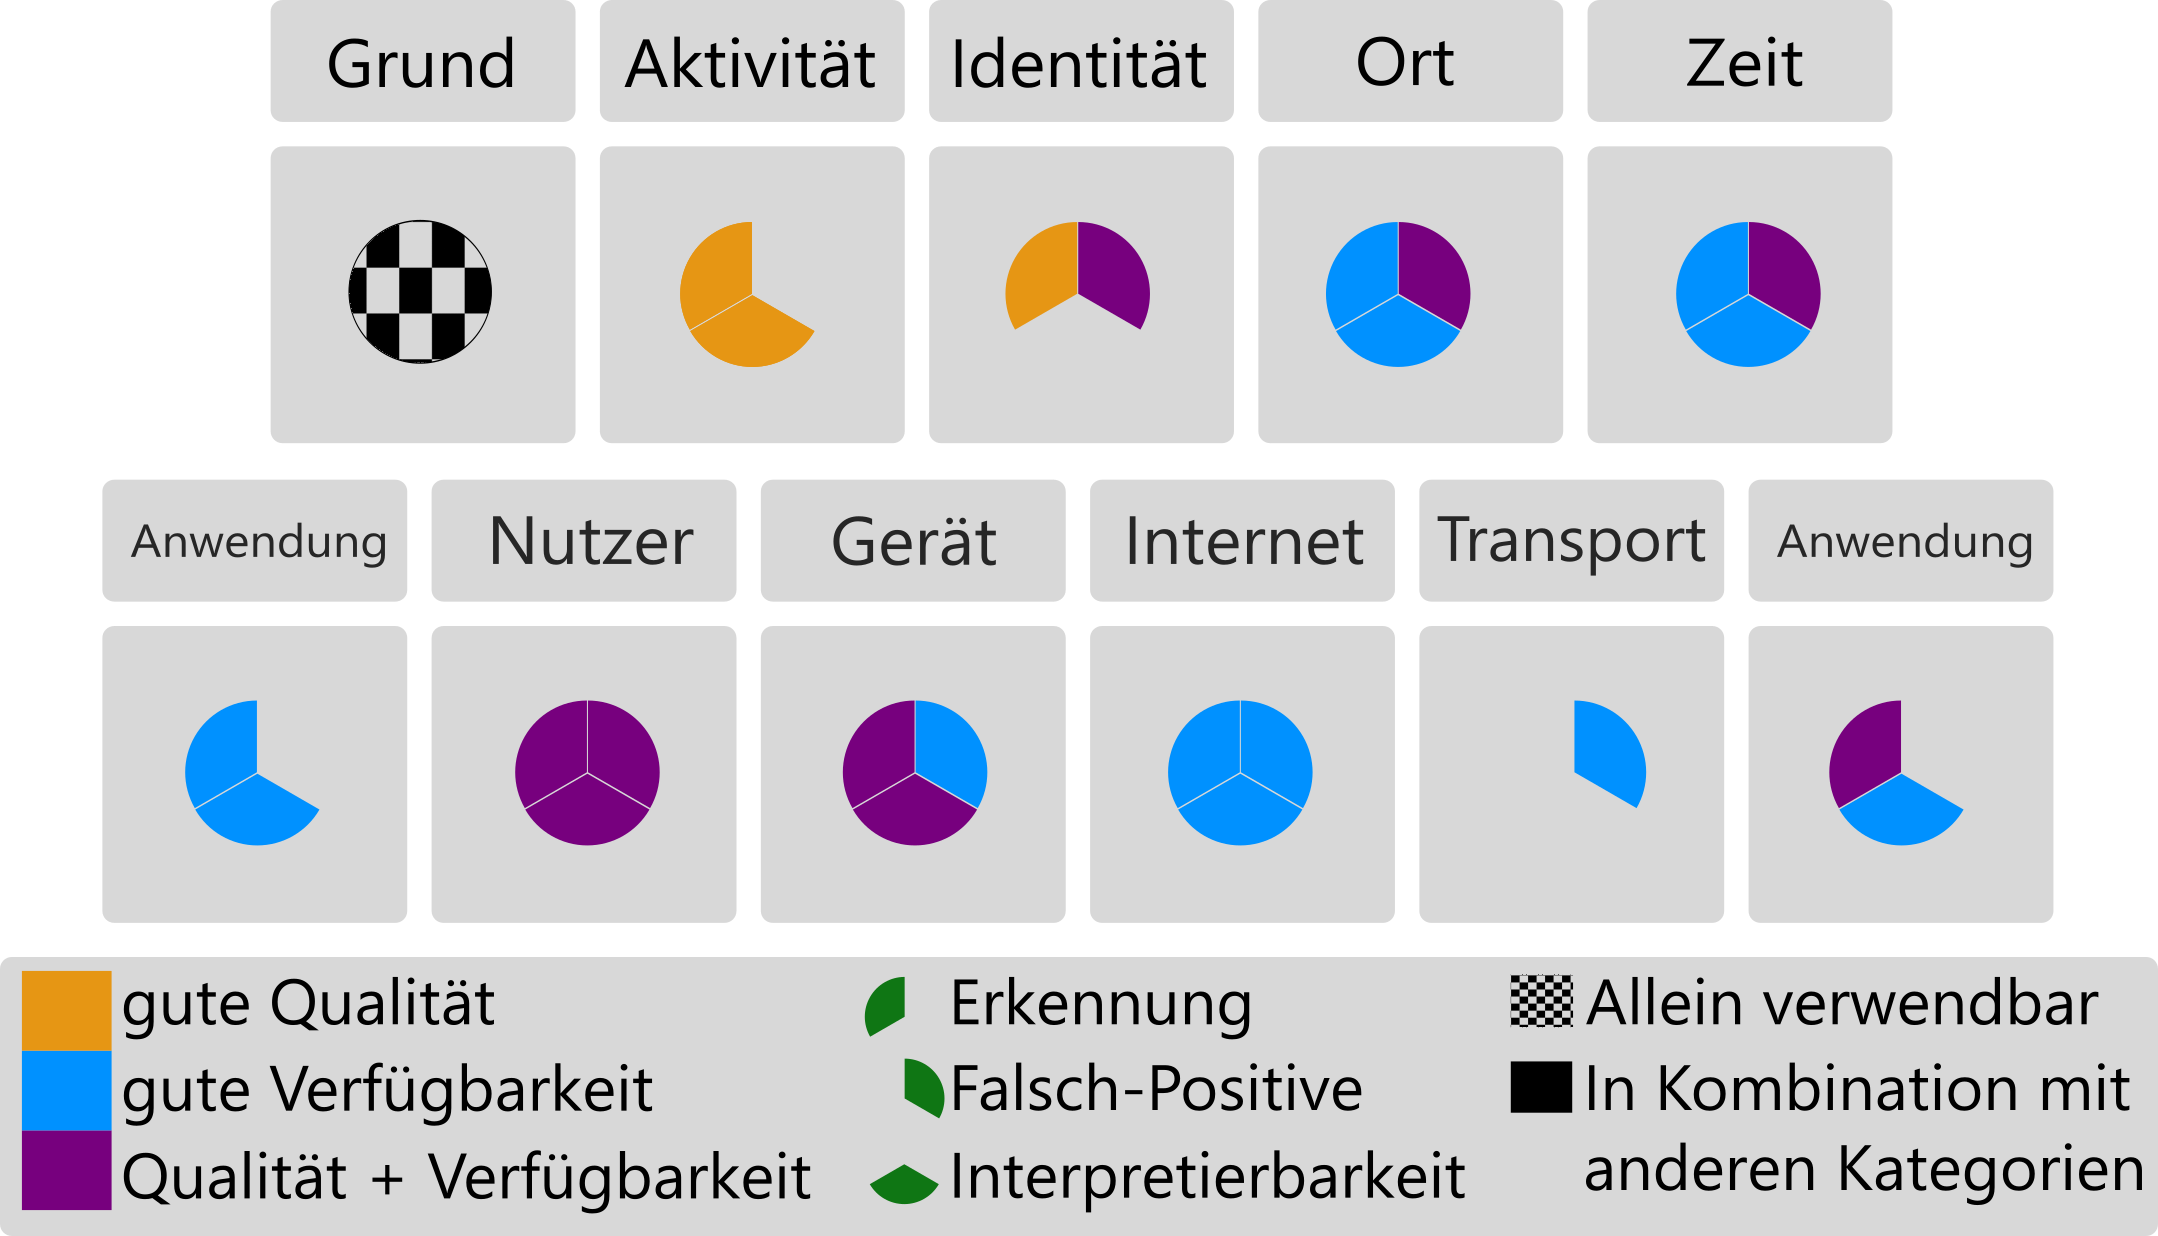
\includegraphics[width=15cm,height=8.5743cm]{Evaluation}
\caption{Evaluation der Taxonomie}
\label{Tax_Ev_1}
\end{figure}

\subsection{Verfügbarkeit der Informationen}
Die Informationen, die im Kapitel \ref{cha:design} beispielhaft als gegeben vorausgesetzt werden, sind in der Praxis unterschiedlich schwer zu akquirieren. Es ist beispielsweise um ein Vielfaches einfacher, korrekt die aktuelle Uhrzeit zu ermitteln als den Grund dafür, das ein Nutzer eine Aktion ausführt, zu bestimmen. Auch sind einige Informationen für die Funktionalität des Netzwerkes und der Kommunikation zwingend notwendig, andere hingegen sind optional oder auf bestimmten Systemen nicht vorhanden.
\subsubsection{Anwendungsfälle}
Die Informationen, die mittels Zeek-Agent direkt vom Host abgefragt werden, sind, da sie ohnehin zum korrekten Betrieb des Systems in der Praxis gebraucht werden, stets verfügbar. Einzig die Zeit, die eine Zeek-Agent-Instanz für eine Antwort benötigt, hat sich bei komplexeren Anfragen oder zu langsamer Hardware als problematisch erwiesen. Es ist also weniger ein Problem, dass Informationen generell nicht vorhanden sind, sondern lediglich nicht ausreichend schnell zur Verfügung gestellt werden können. Im Fall der verwendeten Ports (\ref{Code_4}) führte die Komplexität der an den Zeek-Agent gesendeten Anfrage dazu, das eine Antwort mitunter erst eintraf, nachdem schon zum Hostsystem zugehöriger Netzwerkverkehr bearbeitet wurde. Dies kann vor allem in Netzwerken mit einem hohen Durchsatz und langsam antwortenden Hostsystemen zu fälschlicherweise geblocktem Verkehr führen. Zu einem gewissen Grad lies sich diese Problematik mit festem Scheduling einzelner Events umgehen. Das Scheduling verschiedener Ereignisse mit teilweise asynchronen Antworten wirft allerdings neue Probleme auf. Es empfiehlt sich deshalb, statt eines großen komplexen Skripts mehrere kleinere Skripte zu verwenden, um Leistungseinbrüche zu vermeiden. Dieser modulare Ansatz hat außerdem den Vorteil, dass sich die Menge an Ergebnissen, die miteinander in Bezug gesetzt werden können, vergrößert. So können über einen längeren Zeitraum oder mehrere Geräte verteilte Angriffe noch besser erkannt werden, als wenn lediglich Kontextsensitivität allein verwendet wird.
\subsection{Qualität der Informationen}
Auch die Qualität der Informationen ist in der Praxis limitiert. Genauigkeit und Korrektheit der Informationen sind teilweise stark unterschiedlich. Auch die Vertrauenswürdigkeit und Aktualität der Daten variiert. Es kann im Allgemeinen davon ausgegangen werden, dass Informationen, die von einem Host, der sich im eigenen Netz befindet, stammen, nicht manipuliert sind. Netzwerkverkehr, der von außerhalb das Netzwerk erreicht, ist mit einer höheren Wahrscheinlichkeit verfälscht, gerade wenn die verwendeten Kommunikationsprotokolle und deren Struktur keine inhärenten Möglichkeiten bieten, Informationen oder die Seriosität des Senders zu prüfen.
%\subsection{Anwendungsfälle}
Der momentan limitierende Faktor im Fall der Beispielskripte sind die mit Zeek-Agent Kategorien von abfragbaren Daten. In einer früheren Version des Zeek-Agent bestand die Option, externe Tools wie osquery \footnote{https://osquery.io/} welches zum gegenwärtigen Zeitpunkt für Linux, statt der 7 SQl-Tabellen des Zeek-Agents, 154 Tabellen zur Verfügung stellt \footnote{https://osquery.io/schema/5.5.1/}, anzufragen und damit eine wesentlich größere Menge an Informationen als im momentanen Entwicklungsstand verwenden zu können. Dieser Ansatz wurde allerdings von den Entwicklern aufgrund der zu hohen Komplexität verworfen. Das limitiert in manchen Fällen die abdeckbaren Anwendungsfälle. Nichtsdestotrotz deckt Zeek-Agent in Kombination mit Zeek die im Kapitel \ref{cha:design} vorgeschlagenen Kategorien in ihren Grundzügen sofern möglich, weitestgehend ab.
Bestenfalls stammen Informationen von einer allgemein vertrauenswürdigen Quelle. Außerhalb des Netzwerkes kann das, wie im Skript \ref{Code_5}, zum Beispiel ein autoritativen DNS-Nameserver sein. Innerhalb des Systems sind das Informationen, auf die ein Endnutzer ohne erweiterte Rechte nur begrenzten oder keinen Einfluss ausüben kann oder das meist ohne bewusstes Zutun, wie beispielsweise im Skript \ref{Code_4} die Wahl des Ports geschieht. Damit ist solch ein Datenpunkt ein guter Indikator, um potenziell auffälligen Netzwerkverkehr zu identifizieren.
\section{Leistungsverbesserung}
Die drei Anwendungsbeispiele haben gezeigt, das ein Kontext sowohl die Erkennung von Angriffen und die Rate an Falsch-positiven als auch die Interpretierbarkeit des Geschehens im Netzwerk verbessert.
%TODO